\documentclass[twoside]{article}

% Packages required by doxygen
\usepackage{fixltx2e}
\usepackage{calc}
\usepackage{doxygen}
\usepackage[export]{adjustbox} % also loads graphicx
\usepackage{graphicx}
\usepackage[utf8]{inputenc}
\usepackage{makeidx}
\usepackage{multicol}
\usepackage{multirow}
\PassOptionsToPackage{warn}{textcomp}
\usepackage{textcomp}
\usepackage[nointegrals]{wasysym}
\usepackage[table]{xcolor}

% Font selection
\usepackage[T1]{fontenc}
\usepackage[scaled=.90]{helvet}
\usepackage{courier}
\usepackage{amssymb}
\usepackage{sectsty}
\renewcommand{\familydefault}{\sfdefault}
\allsectionsfont{%
  \fontseries{bc}\selectfont%
  \color{darkgray}%
}
\renewcommand{\DoxyLabelFont}{%
  \fontseries{bc}\selectfont%
  \color{darkgray}%
}
\newcommand{\+}{\discretionary{\mbox{\scriptsize$\hookleftarrow$}}{}{}}

% Page & text layout
\usepackage{geometry}
\geometry{%
  a4paper,%
  top=2.5cm,%
  bottom=2.5cm,%
  left=2.5cm,%
  right=2.5cm%
}
\tolerance=750
\hfuzz=15pt
\hbadness=750
\setlength{\emergencystretch}{15pt}
\setlength{\parindent}{0cm}
\setlength{\parskip}{3ex plus 2ex minus 2ex}
\makeatletter
\renewcommand{\paragraph}{%
  \@startsection{paragraph}{4}{0ex}{-1.0ex}{1.0ex}{%
    \normalfont\normalsize\bfseries\SS@parafont%
  }%
}
\renewcommand{\subparagraph}{%
  \@startsection{subparagraph}{5}{0ex}{-1.0ex}{1.0ex}{%
    \normalfont\normalsize\bfseries\SS@subparafont%
  }%
}
\makeatother

% Headers & footers
\usepackage{fancyhdr}
\pagestyle{fancyplain}
\fancyhead[LE]{\fancyplain{}{\bfseries\thepage}}
\fancyhead[CE]{\fancyplain{}{}}
\fancyhead[RE]{\fancyplain{}{\bfseries\leftmark}}
\fancyhead[LO]{\fancyplain{}{\bfseries\rightmark}}
\fancyhead[CO]{\fancyplain{}{}}
\fancyhead[RO]{\fancyplain{}{\bfseries\thepage}}
\fancyfoot[LE]{\fancyplain{}{}}
\fancyfoot[CE]{\fancyplain{}{}}
\fancyfoot[RE]{\fancyplain{}{\bfseries\scriptsize Generated by Doxygen }}
\fancyfoot[LO]{\fancyplain{}{\bfseries\scriptsize Generated by Doxygen }}
\fancyfoot[CO]{\fancyplain{}{}}
\fancyfoot[RO]{\fancyplain{}{}}
\renewcommand{\footrulewidth}{0.4pt}
\renewcommand{\sectionmark}[1]{%
  \markright{\thesection\ #1}%
}

% Indices & bibliography
\usepackage{natbib}
\usepackage[titles]{tocloft}
\setcounter{tocdepth}{3}
\setcounter{secnumdepth}{5}
\makeindex

% Hyperlinks (required, but should be loaded last)
\usepackage{ifpdf}
\ifpdf
  \usepackage[pdftex,pagebackref=true]{hyperref}
\else
  \usepackage[ps2pdf,pagebackref=true]{hyperref}
\fi
\hypersetup{%
  colorlinks=true,%
  linkcolor=blue,%
  citecolor=blue,%
  unicode%
}

% Custom commands
\newcommand{\clearemptydoublepage}{%
  \newpage{\pagestyle{empty}\cleardoublepage}%
}

\usepackage{caption}
\captionsetup{labelsep=space,justification=centering,font={bf},singlelinecheck=off,skip=4pt,position=top}

%===== C O N T E N T S =====

\begin{document}

% Titlepage & ToC
\hypersetup{pageanchor=false,
             bookmarksnumbered=true,
             pdfencoding=unicode
            }
\pagenumbering{alph}
\begin{titlepage}
\vspace*{7cm}
\begin{center}%
{\Large Proyecto para prueba de Doxygen }\\
\vspace*{1cm}
{\large Generated by Doxygen 1.8.13}\\
\end{center}
\end{titlepage}
\pagenumbering{roman}
\tableofcontents
\pagenumbering{arabic}
\hypersetup{pageanchor=true}

%--- Begin generated contents ---
\section{File Index}
\doxysubsection{File List}
Here is a list of all files with brief descriptions\+:\begin{DoxyCompactList}
\item\contentsline{section}{\mbox{\hyperlink{fibonacci__main_8cc}{fibonacci\+\_\+main.\+cc}} }{\pageref{fibonacci__main_8cc}}{}
\item\contentsline{section}{\mbox{\hyperlink{fibonacci__sum_8cc}{fibonacci\+\_\+sum.\+cc}} }{\pageref{fibonacci__sum_8cc}}{}
\item\contentsline{section}{\mbox{\hyperlink{fibonacci__sum_8h}{fibonacci\+\_\+sum.\+h}} }{\pageref{fibonacci__sum_8h}}{}
\end{DoxyCompactList}

\section{File Documentation}
\hypertarget{fibonacci__main_8cc}{}\subsection{fibonacci\+\_\+main.\+cc File Reference}
\label{fibonacci__main_8cc}\index{fibonacci\+\_\+main.\+cc@{fibonacci\+\_\+main.\+cc}}
{\ttfamily \#include $<$iostream$>$}\newline
{\ttfamily \#include $<$cstdlib$>$}\newline
{\ttfamily \#include \char`\"{}fibonacci\+\_\+sum.\+h\char`\"{}}\newline
Include dependency graph for fibonacci\+\_\+main.\+cc\+:
\nopagebreak
\begin{figure}[H]
\begin{center}
\leavevmode
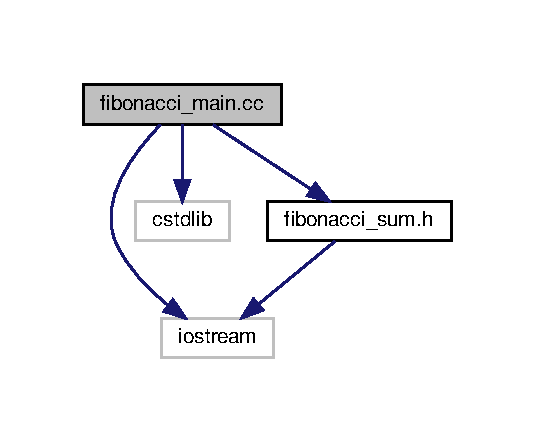
\includegraphics[width=257pt]{fibonacci__main_8cc__incl}
\end{center}
\end{figure}
\subsubsection*{Functions}
\begin{DoxyCompactItemize}
\item 
int \hyperlink{fibonacci__main_8cc_a0ddf1224851353fc92bfbff6f499fa97}{main} (int argc, char $\ast$argv\mbox{[}$\,$\mbox{]})
\begin{DoxyCompactList}\small\item\em Universidad de La Laguna Escuela Superior de Ingeniería y Tecnología Grado en Ingeniería Informática Informática Básica. \end{DoxyCompactList}\end{DoxyCompactItemize}


\subsubsection{Function Documentation}
\mbox{\Hypertarget{fibonacci__main_8cc_a0ddf1224851353fc92bfbff6f499fa97}\label{fibonacci__main_8cc_a0ddf1224851353fc92bfbff6f499fa97}} 
\index{fibonacci\+\_\+main.\+cc@{fibonacci\+\_\+main.\+cc}!main@{main}}
\index{main@{main}!fibonacci\+\_\+main.\+cc@{fibonacci\+\_\+main.\+cc}}
\paragraph{\texorpdfstring{main()}{main()}}
{\footnotesize\ttfamily int main (\begin{DoxyParamCaption}\item[{int}]{argc,  }\item[{char $\ast$}]{argv\mbox{[}$\,$\mbox{]} }\end{DoxyParamCaption})}



Universidad de La Laguna Escuela Superior de Ingeniería y Tecnología Grado en Ingeniería Informática Informática Básica. 

\begin{DoxyAuthor}{Author}
F. de Sande 
\end{DoxyAuthor}
\begin{DoxyDate}{Date}
7.\+nov.\+2020 Cada nuevo término de la serie de Fibonacci se genera sumando los dos anteriores. Comenzando con 0 y 1, los primeros 10 términos serán\+: 0, 1, 1, 2, 3, 5, 8, 13, 21, 34 Desarrolle en C++ un programa que calcule la suma de todos los términos de valor par de la serie que sean menores que 1000. 
\end{DoxyDate}
\begin{DoxySeeAlso}{See also}
\href{https://docs.google.com/document/d/1-3hTIVf8tPrbn9u0vs0Cm2IGyX1XBgv8hReVU0KOSUQ/edit?usp=sharing}{\tt https\+://docs.\+google.\+com/document/d/1-\/3h\+T\+I\+Vf8t\+Prbn9u0vs0\+Cm2\+I\+Gy\+X1\+X\+Bgv8h\+Re\+V\+U0\+K\+O\+S\+U\+Q/edit?usp=sharing} 

stoi \href{http://www.cplusplus.com/reference/string/stoi/}{\tt http\+://www.\+cplusplus.\+com/reference/string/stoi/} An Object Oriented Version of the program\+: 

\href{https://stackoverflow.com/questions/21360694/sum-of-even-fibonacci-numbers-under-1000exit}{\tt https\+://stackoverflow.\+com/questions/21360694/sum-\/of-\/even-\/fibonacci-\/numbers-\/under-\/1000exit} Main function 
\end{DoxySeeAlso}

\begin{DoxyParams}[1]{Parameters}
\mbox{\tt in}  & {\em argc} & Number of command line parameters \\
\hline
\mbox{\tt in}  & {\em argv} & Vector containing (char$\ast$) the parameters \\
\hline
\end{DoxyParams}


Definition at line 29 of file fibonacci\+\_\+main.\+cc.



References fibonacci\+\_\+sum(), and Usage().


\begin{DoxyCode}
29                                   \{
30   \hyperlink{fibonacci__sum_8cc_aeac332c082069f54e8769d311dd2049d}{Usage}(argc, argv);
31   std::string limit = argv[1];
32   \textcolor{keyword}{const} \textcolor{keywordtype}{size\_t} kLimit = stoi(limit);
33   std::cout << \textcolor{stringliteral}{"Sum: "} << \hyperlink{fibonacci__sum_8cc_adbea092e9a2442d7c23f17af8285b7d2}{fibonacci\_sum}(kLimit) << std::endl; 
34   \textcolor{keywordflow}{return} 0;
35 \}
\end{DoxyCode}
Here is the call graph for this function\+:
\nopagebreak
\begin{figure}[H]
\begin{center}
\leavevmode
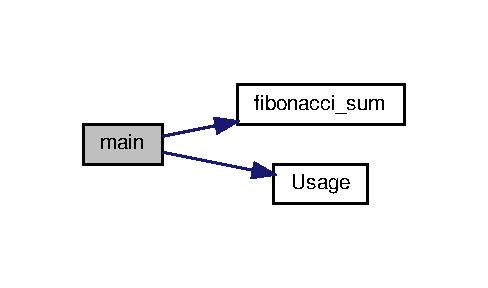
\includegraphics[width=234pt]{fibonacci__main_8cc_a0ddf1224851353fc92bfbff6f499fa97_cgraph}
\end{center}
\end{figure}

\hypertarget{fibonacci__sum_8cc}{}\subsection{fibonacci\+\_\+sum.\+cc File Reference}
\label{fibonacci__sum_8cc}\index{fibonacci\+\_\+sum.\+cc@{fibonacci\+\_\+sum.\+cc}}
{\ttfamily \#include $<$iostream$>$}\newline
{\ttfamily \#include $<$cstdlib$>$}\newline
{\ttfamily \#include \char`\"{}fibonacci\+\_\+sum.\+h\char`\"{}}\newline
Include dependency graph for fibonacci\+\_\+sum.\+cc\+:
\nopagebreak
\begin{figure}[H]
\begin{center}
\leavevmode
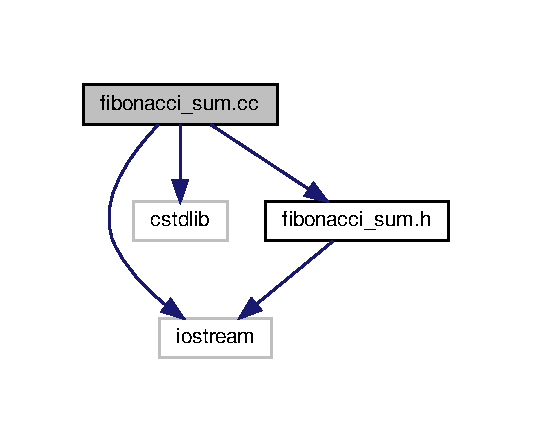
\includegraphics[width=256pt]{fibonacci__sum_8cc__incl}
\end{center}
\end{figure}
\subsubsection*{Functions}
\begin{DoxyCompactItemize}
\item 
void \hyperlink{fibonacci__sum_8cc_aeac332c082069f54e8769d311dd2049d}{Usage} (int argc, char $\ast$argv\mbox{[}$\,$\mbox{]})
\begin{DoxyCompactList}\small\item\em Universidad de La Laguna Escuela Superior de Ingeniería y Tecnología Grado en Ingeniería Informática Informática Básica. \end{DoxyCompactList}\item 
size\+\_\+t \hyperlink{fibonacci__sum_8cc_adbea092e9a2442d7c23f17af8285b7d2}{fibonacci\+\_\+sum} (const size\+\_\+t k\+Limit)
\begin{DoxyCompactList}\small\item\em Devuelve el valor de la suma de todos los términos de valor par de la serie de Fibonacci menores que k\+Limit. \end{DoxyCompactList}\end{DoxyCompactItemize}


\subsubsection{Function Documentation}
\mbox{\Hypertarget{fibonacci__sum_8cc_adbea092e9a2442d7c23f17af8285b7d2}\label{fibonacci__sum_8cc_adbea092e9a2442d7c23f17af8285b7d2}} 
\index{fibonacci\+\_\+sum.\+cc@{fibonacci\+\_\+sum.\+cc}!fibonacci\+\_\+sum@{fibonacci\+\_\+sum}}
\index{fibonacci\+\_\+sum@{fibonacci\+\_\+sum}!fibonacci\+\_\+sum.\+cc@{fibonacci\+\_\+sum.\+cc}}
\paragraph{\texorpdfstring{fibonacci\+\_\+sum()}{fibonacci\_sum()}}
{\footnotesize\ttfamily size\+\_\+t fibonacci\+\_\+sum (\begin{DoxyParamCaption}\item[{const size\+\_\+t}]{k\+Limit }\end{DoxyParamCaption})}



Devuelve el valor de la suma de todos los términos de valor par de la serie de Fibonacci menores que k\+Limit. 


\begin{DoxyParams}[1]{Parameters}
\mbox{\tt in}  & {\em k\+Limit.} & Se suman los términos pares menores que k\+Limit \\
\hline
\end{DoxyParams}
\begin{DoxyReturn}{Returns}
La suma de los términos pares menores que k\+Limit 
\end{DoxyReturn}


Definition at line 52 of file fibonacci\+\_\+sum.\+cc.



Referenced by main().


\begin{DoxyCode}
52                                           \{
53   \textcolor{keywordtype}{size\_t} second\_to\_last\{0\},  \textcolor{comment}{// Second to last term}
54            last\{1\},          \textcolor{comment}{// Last term generated}
55            new\_term;         \textcolor{comment}{// New term of the serie}
56   \textcolor{keywordtype}{size\_t} \textcolor{keywordtype}{long} sum\{0\};        \textcolor{comment}{// Accumulated sum of the terms}
57 
58   \textcolor{keywordflow}{do} \{
59     new\_term = last + second\_to\_last;
60     \textcolor{keywordflow}{if} (new\_term % 2 == 0) \{
61       sum += new\_term;
62     \}
63     \textcolor{comment}{// Uncomment for debug: print each new term}
64     \textcolor{comment}{// std::cout << "Term: " << new\_term << std::endl;}
65     second\_to\_last = last;
66     last = new\_term;
67   \} \textcolor{keywordflow}{while} (new\_term < kLimit);
68   \textcolor{keywordflow}{return} sum;
69 \}
\end{DoxyCode}
Here is the caller graph for this function\+:
\nopagebreak
\begin{figure}[H]
\begin{center}
\leavevmode
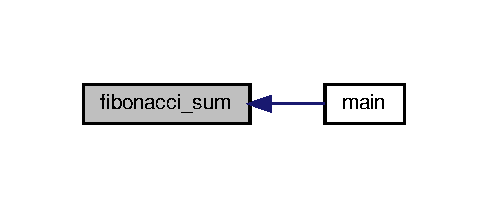
\includegraphics[width=234pt]{fibonacci__sum_8cc_adbea092e9a2442d7c23f17af8285b7d2_icgraph}
\end{center}
\end{figure}
\mbox{\Hypertarget{fibonacci__sum_8cc_aeac332c082069f54e8769d311dd2049d}\label{fibonacci__sum_8cc_aeac332c082069f54e8769d311dd2049d}} 
\index{fibonacci\+\_\+sum.\+cc@{fibonacci\+\_\+sum.\+cc}!Usage@{Usage}}
\index{Usage@{Usage}!fibonacci\+\_\+sum.\+cc@{fibonacci\+\_\+sum.\+cc}}
\paragraph{\texorpdfstring{Usage()}{Usage()}}
{\footnotesize\ttfamily void Usage (\begin{DoxyParamCaption}\item[{int}]{argc,  }\item[{char $\ast$}]{argv\mbox{[}$\,$\mbox{]} }\end{DoxyParamCaption})}



Universidad de La Laguna Escuela Superior de Ingeniería y Tecnología Grado en Ingeniería Informática Informática Básica. 

\begin{DoxyAuthor}{Author}
F. de Sande 
\end{DoxyAuthor}
\begin{DoxyDate}{Date}
7.\+nov.\+2020 Cada nuevo término de la serie de Fibonacci se genera sumando los dos anteriores. Comenzando con 0 y 1, los primeros 10 términos serán\+: 0, 1, 1, 2, 3, 5, 8, 13, 21, 34 Desarrolle en C++ un programa que calcule la suma de todos los términos de valor par de la serie que sean menores que 1000. 
\end{DoxyDate}
\begin{DoxySeeAlso}{See also}
\href{https://docs.google.com/document/d/1-3hTIVf8tPrbn9u0vs0Cm2IGyX1XBgv8hReVU0KOSUQ/edit?usp=sharing}{\tt https\+://docs.\+google.\+com/document/d/1-\/3h\+T\+I\+Vf8t\+Prbn9u0vs0\+Cm2\+I\+Gy\+X1\+X\+Bgv8h\+Re\+V\+U0\+K\+O\+S\+U\+Q/edit?usp=sharing} 

stoi \href{http://www.cplusplus.com/reference/string/stoi/}{\tt http\+://www.\+cplusplus.\+com/reference/string/stoi/} An Object Oriented Version of the program\+: 

\href{https://stackoverflow.com/questions/21360694/sum-of-even-fibonacci-numbers-under-1000Muestra}{\tt https\+://stackoverflow.\+com/questions/21360694/sum-\/of-\/even-\/fibonacci-\/numbers-\/under-\/1000\+Muestra} el modo de uso correcto del programa En caso de que el uso no sea el correcto, muestra el mensaje y finaliza la ejecución del programa. El programa precisa un único número natural para su ejecución.
\end{DoxySeeAlso}

\begin{DoxyParams}[1]{Parameters}
\mbox{\tt in}  & {\em argc} & Number of command line parameters \\
\hline
\mbox{\tt in}  & {\em argv} & Vector containing (char$\ast$) the parameters \\
\hline
\end{DoxyParams}


Definition at line 33 of file fibonacci\+\_\+sum.\+cc.



References k\+Help\+Text.



Referenced by main().


\begin{DoxyCode}
33                                    \{
34   \textcolor{keywordflow}{if} (argc != 2) \{
35     std::cout << argv[0] << \textcolor{stringliteral}{": Falta un número natural como parámetro"} << std::endl;
36     std::cout << \textcolor{stringliteral}{"Pruebe "} << argv[0] << \textcolor{stringliteral}{" --help para más información"} << std::endl;
37     exit(EXIT\_SUCCESS);
38   \}
39   std::string parameter\{argv[1]\};
40   \textcolor{keywordflow}{if} (parameter == \textcolor{stringliteral}{"--help"}) \{
41     std::cout << \hyperlink{fibonacci__sum_8h_a08728caac9a53278aea6a3218ae1dfeb}{kHelpText} << std::endl;
42     exit(EXIT\_SUCCESS);
43   \}
44 \}
\end{DoxyCode}
Here is the caller graph for this function\+:
\nopagebreak
\begin{figure}[H]
\begin{center}
\leavevmode
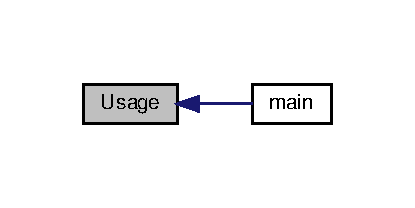
\includegraphics[width=199pt]{fibonacci__sum_8cc_aeac332c082069f54e8769d311dd2049d_icgraph}
\end{center}
\end{figure}

\hypertarget{fibonacci__sum_8h}{}\doxysubsection{fibonacci\+\_\+sum.\+h File Reference}
\label{fibonacci__sum_8h}\index{fibonacci\_sum.h@{fibonacci\_sum.h}}
{\ttfamily \#include $<$iostream$>$}\newline
Include dependency graph for fibonacci\+\_\+sum.\+h\+:\nopagebreak
\begin{figure}[H]
\begin{center}
\leavevmode
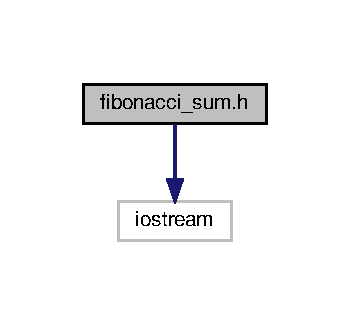
\includegraphics[width=175pt]{fibonacci__sum_8h__incl}
\end{center}
\end{figure}
This graph shows which files directly or indirectly include this file\+:\nopagebreak
\begin{figure}[H]
\begin{center}
\leavevmode
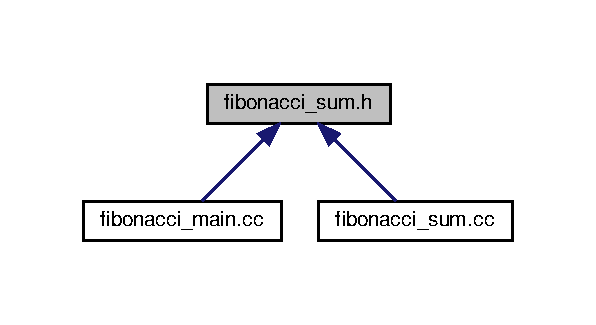
\includegraphics[width=302pt]{fibonacci__sum_8h__dep__incl}
\end{center}
\end{figure}
\doxysubsubsection*{Functions}
\begin{DoxyCompactItemize}
\item 
void \mbox{\hyperlink{fibonacci__sum_8h_aeac332c082069f54e8769d311dd2049d}{Usage}} (int argc, char $\ast$argv\mbox{[}$\,$\mbox{]})
\begin{DoxyCompactList}\small\item\em Universidad de La Laguna Escuela Superior de Ingeniería y Tecnología Grado en Ingeniería Informática Informática Básica. \end{DoxyCompactList}\item 
size\+\_\+t \mbox{\hyperlink{fibonacci__sum_8h_adbea092e9a2442d7c23f17af8285b7d2}{fibonacci\+\_\+sum}} (const size\+\_\+t k\+Limit)
\begin{DoxyCompactList}\small\item\em Devuelve el valor de la suma de todos los términos de valor par de la serie de Fibonacci menores que k\+Limit. \end{DoxyCompactList}\end{DoxyCompactItemize}
\doxysubsubsection*{Variables}
\begin{DoxyCompactItemize}
\item 
const std\+::string \mbox{\hyperlink{fibonacci__sum_8h_a08728caac9a53278aea6a3218ae1dfeb}{k\+Help\+Text}}
\begin{DoxyCompactList}\small\item\em Universidad de La Laguna Escuela Superior de Ingeniería y Tecnología Grado en Ingeniería Informática Informática Básica. \end{DoxyCompactList}\end{DoxyCompactItemize}


\doxysubsubsection{Function Documentation}
\mbox{\Hypertarget{fibonacci__sum_8h_adbea092e9a2442d7c23f17af8285b7d2}\label{fibonacci__sum_8h_adbea092e9a2442d7c23f17af8285b7d2}} 
\index{fibonacci\_sum.h@{fibonacci\_sum.h}!fibonacci\_sum@{fibonacci\_sum}}
\index{fibonacci\_sum@{fibonacci\_sum}!fibonacci\_sum.h@{fibonacci\_sum.h}}
\doxyparagraph{\texorpdfstring{fibonacci\_sum()}{fibonacci\_sum()}}
{\footnotesize\ttfamily size\+\_\+t fibonacci\+\_\+sum (\begin{DoxyParamCaption}\item[{const size\+\_\+t}]{k\+Limit }\end{DoxyParamCaption})}



Devuelve el valor de la suma de todos los términos de valor par de la serie de Fibonacci menores que k\+Limit. 


\begin{DoxyParams}[1]{Parameters}
\mbox{\texttt{ in}}  & {\em k\+Limit.} & Se suman los términos pares menores que k\+Limit \\
\hline
\end{DoxyParams}
\begin{DoxyReturn}{Returns}
La suma de los términos pares menores que k\+Limit 
\end{DoxyReturn}


Definition at line 52 of file fibonacci\+\_\+sum.\+cc.


\begin{DoxyCode}{0}
\DoxyCodeLine{52                                           \{}
\DoxyCodeLine{53   \textcolor{keywordtype}{size\_t} second\_to\_last\{0\},  \textcolor{comment}{// Second to last term}}
\DoxyCodeLine{54            last\{1\},          \textcolor{comment}{// Last term generated}}
\DoxyCodeLine{55            new\_term;         \textcolor{comment}{// New term of the serie}}
\DoxyCodeLine{56   \textcolor{keywordtype}{size\_t} \textcolor{keywordtype}{long} sum\{0\};        \textcolor{comment}{// Accumulated sum of the terms}}
\DoxyCodeLine{57 }
\DoxyCodeLine{58   \textcolor{keywordflow}{do} \{}
\DoxyCodeLine{59     new\_term = last + second\_to\_last;}
\DoxyCodeLine{60     \textcolor{keywordflow}{if} (new\_term \% 2 == 0) \{}
\DoxyCodeLine{61       sum += new\_term;}
\DoxyCodeLine{62     \}}
\DoxyCodeLine{63     \textcolor{comment}{// Uncomment for debug: print each new term}}
\DoxyCodeLine{64     \textcolor{comment}{// std::cout << "Term: " << new\_term << std::endl;}}
\DoxyCodeLine{65     second\_to\_last = last;}
\DoxyCodeLine{66     last = new\_term;}
\DoxyCodeLine{67   \} \textcolor{keywordflow}{while} (new\_term < kLimit);}
\DoxyCodeLine{68   \textcolor{keywordflow}{return} sum;}
\DoxyCodeLine{69 \}}

\end{DoxyCode}


Referenced by main().

Here is the caller graph for this function\+:
\nopagebreak
\begin{figure}[H]
\begin{center}
\leavevmode
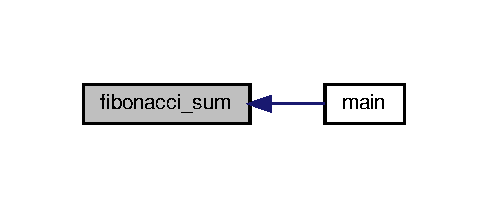
\includegraphics[width=243pt]{fibonacci__sum_8h_adbea092e9a2442d7c23f17af8285b7d2_icgraph}
\end{center}
\end{figure}
\mbox{\Hypertarget{fibonacci__sum_8h_aeac332c082069f54e8769d311dd2049d}\label{fibonacci__sum_8h_aeac332c082069f54e8769d311dd2049d}} 
\index{fibonacci\_sum.h@{fibonacci\_sum.h}!Usage@{Usage}}
\index{Usage@{Usage}!fibonacci\_sum.h@{fibonacci\_sum.h}}
\doxyparagraph{\texorpdfstring{Usage()}{Usage()}}
{\footnotesize\ttfamily void Usage (\begin{DoxyParamCaption}\item[{int}]{argc,  }\item[{char $\ast$}]{argv\mbox{[}$\,$\mbox{]} }\end{DoxyParamCaption})}



Universidad de La Laguna Escuela Superior de Ingeniería y Tecnología Grado en Ingeniería Informática Informática Básica. 

\begin{DoxyAuthor}{Author}
F. de Sande 
\end{DoxyAuthor}
\begin{DoxyDate}{Date}
7.\+nov.\+2020
\end{DoxyDate}
Cada nuevo término de la serie de Fibonacci se genera sumando los dos anteriores. Comenzando con 0 y 1, los primeros 10 términos serán\+: 0, 1, 1, 2, 3, 5, 8, 13, 21, 34 Desarrolle en C++ un programa que calcule la suma de todos los términos de valor par de la serie que sean menores que 1000. \begin{DoxySeeAlso}{See also}
\href{https://docs.google.com/document/d/1-3hTIVf8tPrbn9u0vs0Cm2IGyX1XBgv8hReVU0KOSUQ/edit?usp=sharing}{\texttt{ https\+://docs.\+google.\+com/document/d/1-\/3h\+T\+I\+Vf8t\+Prbn9u0vs0\+Cm2\+I\+Gy\+X1\+X\+Bgv8h\+Re\+V\+U0\+K\+O\+S\+U\+Q/edit?usp=sharing}} 

stoi \href{http://www.cplusplus.com/reference/string/stoi/}{\texttt{ http\+://www.\+cplusplus.\+com/reference/string/stoi/}} An Object Oriented Version of the program\+: 

\href{https://stackoverflow.com/questions/21360694/sum-of-even-fibonacci-numbers-under-1000}{\texttt{ https\+://stackoverflow.\+com/questions/21360694/sum-\/of-\/even-\/fibonacci-\/numbers-\/under-\/1000}} Muestra el modo de uso correcto del programa En caso de que el uso no sea el correcto, muestra el mensaje y finaliza la ejecución del programa. El programa precisa un único número natural para su ejecución.
\end{DoxySeeAlso}

\begin{DoxyParams}[1]{Parameters}
\mbox{\texttt{ in}}  & {\em argc} & Number of command line parameters \\
\hline
\mbox{\texttt{ in}}  & {\em argv} & Vector containing (char$\ast$) the parameters \\
\hline
\end{DoxyParams}


Definition at line 33 of file fibonacci\+\_\+sum.\+cc.


\begin{DoxyCode}{0}
\DoxyCodeLine{33                                    \{}
\DoxyCodeLine{34   \textcolor{keywordflow}{if} (argc != 2) \{}
\DoxyCodeLine{35     std::cout << argv[0] << \textcolor{stringliteral}{": Falta un número natural como parámetro"} << std::endl;}
\DoxyCodeLine{36     std::cout << \textcolor{stringliteral}{"Pruebe "} << argv[0] << \textcolor{stringliteral}{" -\/-\/help para más información"} << std::endl;}
\DoxyCodeLine{37     exit(EXIT\_SUCCESS);}
\DoxyCodeLine{38   \}}
\DoxyCodeLine{39   std::string parameter\{argv[1]\};}
\DoxyCodeLine{40   \textcolor{keywordflow}{if} (parameter == \textcolor{stringliteral}{"-\/-\/help"}) \{}
\DoxyCodeLine{41     std::cout << \mbox{\hyperlink{fibonacci__sum_8h_a08728caac9a53278aea6a3218ae1dfeb}{kHelpText}} << std::endl;}
\DoxyCodeLine{42     exit(EXIT\_SUCCESS);}
\DoxyCodeLine{43   \}}
\DoxyCodeLine{44 \}}

\end{DoxyCode}


References k\+Help\+Text.



Referenced by main().

Here is the caller graph for this function\+:
\nopagebreak
\begin{figure}[H]
\begin{center}
\leavevmode
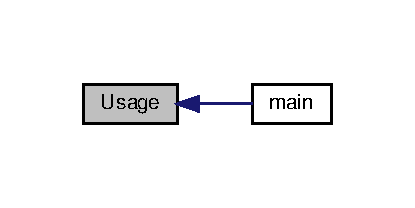
\includegraphics[width=204pt]{fibonacci__sum_8h_aeac332c082069f54e8769d311dd2049d_icgraph}
\end{center}
\end{figure}


\doxysubsubsection{Variable Documentation}
\mbox{\Hypertarget{fibonacci__sum_8h_a08728caac9a53278aea6a3218ae1dfeb}\label{fibonacci__sum_8h_a08728caac9a53278aea6a3218ae1dfeb}} 
\index{fibonacci\_sum.h@{fibonacci\_sum.h}!kHelpText@{kHelpText}}
\index{kHelpText@{kHelpText}!fibonacci\_sum.h@{fibonacci\_sum.h}}
\doxyparagraph{\texorpdfstring{kHelpText}{kHelpText}}
{\footnotesize\ttfamily const std\+::string k\+Help\+Text}

{\bfseries Initial value\+:}
\begin{DoxyCode}{0}
\DoxyCodeLine{= \textcolor{stringliteral}{"Este programa calcula la suma de todos los términos pares de la \(\backslash\)}}
\DoxyCodeLine{\textcolor{stringliteral}{serie de Fibonacci que sean menores que un valor, que el usuario \(\backslash\)}}
\DoxyCodeLine{\textcolor{stringliteral}{ha de introducir por línea de comandos para la ejecución del programa"}}

\end{DoxyCode}


Universidad de La Laguna Escuela Superior de Ingeniería y Tecnología Grado en Ingeniería Informática Informática Básica. 

\begin{DoxyAuthor}{Author}
F. de Sande 
\end{DoxyAuthor}
\begin{DoxyDate}{Date}
7.\+nov.\+2020
\end{DoxyDate}
Definitions 

Definition at line 15 of file fibonacci\+\_\+sum.\+h.



Referenced by Usage().


%--- End generated contents ---

% Index
\newpage
\phantomsection
\clearemptydoublepage
\addcontentsline{toc}{section}{Index}
\printindex

\end{document}
